\begin{enumerate}[label=\arabic*.,ref=\thesection.\theenumi]
\numberwithin{equation}{enumi}
\item List the various components used to implement receiver.
\\
\solution
\\
\begin{table}[!ht]
  \centering
  %%%%%%%%%%%%%%%%%%%%%%%%%%%%%%%%%%%%%%%%%%%%%%%%%%%%%%%%%%%%%%%%%%%%%%
%%                                                                  %%
%%  This is the header of a LaTeX2e file exported from Gnumeric.    %%
%%                                                                  %%
%%  This file can be compiled as it stands or included in another   %%
%%  LaTeX document. The table is based on the longtable package so  %%
%%  the longtable options (headers, footers...) can be set in the   %%
%%  preamble section below (see PRAMBLE).                           %%
%%                                                                  %%
%%  To include the file in another, the following two lines must be %%
%%  in the including file:                                          %%
%%        \def\inputGnumericTable{}                                 %%
%%  at the beginning of the file and:                               %%
%%        \input{name-of-this-file.tex}                             %%
%%  where the table is to be placed. Note also that the including   %%
%%  file must use the following packages for the table to be        %%
%%  rendered correctly:                                             %%
%%    \usepackage[latin1]{inputenc}                                 %%
%%    \usepackage{color}                                            %%
%%    \usepackage{array}                                            %%
%%    \usepackage{longtable}                                        %%
%%    \usepackage{calc}                                             %%
%%    \usepackage{multirow}                                         %%
%%    \usepackage{hhline}                                           %%
%%    \usepackage{ifthen}                                           %%
%%  optionally (for landscape tables embedded in another document): %%
%%    \usepackage{lscape}                                           %%
%%                                                                  %%
%%%%%%%%%%%%%%%%%%%%%%%%%%%%%%%%%%%%%%%%%%%%%%%%%%%%%%%%%%%%%%%%%%%%%%



%%  This section checks if we are begin input into another file or  %%
%%  the file will be compiled alone. First use a macro taken from   %%
%%  the TeXbook ex 7.7 (suggestion of Han-Wen Nienhuys).            %%
\def\ifundefined#1{\expandafter\ifx\csname#1\endcsname\relax}


%%  Check for the \def token for inputed files. If it is not        %%
%%  defined, the file will be processed as a standalone and the     %%
%%  preamble will be used.                                          %%
\ifundefined{inputGnumericTable}

%%  We must be able to close or not the document at the end.        %%
	\def\gnumericTableEnd{\end{document}}


%%%%%%%%%%%%%%%%%%%%%%%%%%%%%%%%%%%%%%%%%%%%%%%%%%%%%%%%%%%%%%%%%%%%%%
%%                                                                  %%
%%  This is the PREAMBLE. Change these values to get the right      %%
%%  paper size and other niceties.                                  %%
%%                                                                  %%
%%%%%%%%%%%%%%%%%%%%%%%%%%%%%%%%%%%%%%%%%%%%%%%%%%%%%%%%%%%%%%%%%%%%%%

	\documentclass[12pt%
			  %,landscape%
                    ]{report}
       \usepackage[latin1]{inputenc}
       \usepackage{fullpage}
       \usepackage{color}
       \usepackage{array}
       \usepackage{longtable}
       \usepackage{calc}
       \usepackage{multirow}
       \usepackage{hhline}
       \usepackage{ifthen}

	\begin{document}


%%  End of the preamble for the standalone. The next section is for %%
%%  documents which are included into other LaTeX2e files.          %%
\else

%%  We are not a stand alone document. For a regular table, we will %%
%%  have no preamble and only define the closing to mean nothing.   %%
    \def\gnumericTableEnd{}

%%  If we want landscape mode in an embedded document, comment out  %%
%%  the line above and uncomment the two below. The table will      %%
%%  begin on a new page and run in landscape mode.                  %%
%       \def\gnumericTableEnd{\end{landscape}}
%       \begin{landscape}


%%  End of the else clause for this file being \input.              %%
\fi

%%%%%%%%%%%%%%%%%%%%%%%%%%%%%%%%%%%%%%%%%%%%%%%%%%%%%%%%%%%%%%%%%%%%%%
%%                                                                  %%
%%  The rest is the gnumeric table, except for the closing          %%
%%  statement. Changes below will alter the table's appearance.     %%
%%                                                                  %%
%%%%%%%%%%%%%%%%%%%%%%%%%%%%%%%%%%%%%%%%%%%%%%%%%%%%%%%%%%%%%%%%%%%%%%

\providecommand{\gnumericmathit}[1]{#1} 
%%  Uncomment the next line if you would like your numbers to be in %%
%%  italics if they are italizised in the gnumeric table.           %%
%\renewcommand{\gnumericmathit}[1]{\mathit{#1}}
\providecommand{\gnumericPB}[1]%
{\let\gnumericTemp=\\#1\let\\=\gnumericTemp\hspace{0pt}}
 \ifundefined{gnumericTableWidthDefined}
        \newlength{\gnumericTableWidth}
        \newlength{\gnumericTableWidthComplete}
        \newlength{\gnumericMultiRowLength}
        \global\def\gnumericTableWidthDefined{}
 \fi
%% The following setting protects this code from babel shorthands.  %%
 \ifthenelse{\isundefined{\languageshorthands}}{}{\languageshorthands{english}}
%%  The default table format retains the relative column widths of  %%
%%  gnumeric. They can easily be changed to c, r or l. In that case %%
%%  you may want to comment out the next line and uncomment the one %%
%%  thereafter                                                      %%
\providecommand\gnumbox{\makebox[0pt]}
%%\providecommand\gnumbox[1][]{\makebox}

%% to adjust positions in multirow situations                       %%
\setlength{\bigstrutjot}{\jot}
\setlength{\extrarowheight}{\doublerulesep}

%%  The \setlongtables command keeps column widths the same across  %%
%%  pages. Simply comment out next line for varying column widths.  %%
\setlongtables

\setlength\gnumericTableWidth{%
	98pt+%
	215pt+%
	53pt+%
	53pt+%
0pt}
\def\gumericNumCols{4}
\setlength\gnumericTableWidthComplete{\gnumericTableWidth+%
         \tabcolsep*\gumericNumCols*2+\arrayrulewidth*\gumericNumCols}
\ifthenelse{\lengthtest{\gnumericTableWidthComplete > \linewidth}}%
         {\def\gnumericScale{1*\ratio{\linewidth-%
                        \tabcolsep*\gumericNumCols*2-%
                        \arrayrulewidth*\gumericNumCols}%
{\gnumericTableWidth}}}%
{\def\gnumericScale{1}}

%%%%%%%%%%%%%%%%%%%%%%%%%%%%%%%%%%%%%%%%%%%%%%%%%%%%%%%%%%%%%%%%%%%%%%
%%                                                                  %%
%% The following are the widths of the various columns. We are      %%
%% defining them here because then they are easier to change.       %%
%% Depending on the cell formats we may use them more than once.    %%
%%                                                                  %%
%%%%%%%%%%%%%%%%%%%%%%%%%%%%%%%%%%%%%%%%%%%%%%%%%%%%%%%%%%%%%%%%%%%%%%

\ifthenelse{\isundefined{\gnumericColA}}{\newlength{\gnumericColA}}{}\settowidth{\gnumericColA}{\begin{tabular}{@{}p{98pt*\gnumericScale}@{}}x\end{tabular}}
\ifthenelse{\isundefined{\gnumericColB}}{\newlength{\gnumericColB}}{}\settowidth{\gnumericColB}{\begin{tabular}{@{}p{215pt*\gnumericScale}@{}}x\end{tabular}}
\ifthenelse{\isundefined{\gnumericColC}}{\newlength{\gnumericColC}}{}\settowidth{\gnumericColC}{\begin{tabular}{@{}p{53pt*\gnumericScale}@{}}x\end{tabular}}
\ifthenelse{\isundefined{\gnumericColD}}{\newlength{\gnumericColD}}{}\settowidth{\gnumericColD}{\begin{tabular}{@{}p{53pt*\gnumericScale}@{}}x\end{tabular}}

\begin{longtable}[c]{%
	b{\gnumericColA}%
	b{\gnumericColB}%
	b{\gnumericColC}%
	b{\gnumericColD}%
	}

%%%%%%%%%%%%%%%%%%%%%%%%%%%%%%%%%%%%%%%%%%%%%%%%%%%%%%%%%%%%%%%%%%%%%%
%%  The longtable options. (Caption, headers... see Goosens, p.124) %%
%	\caption{The Table Caption.}             \\	%
% \hline	% Across the top of the table.
%%  The rest of these options are table rows which are placed on    %%
%%  the first, last or every page. Use \multicolumn if you want.    %%

%%  Header for the first page.                                      %%
%	\multicolumn{4}{c}{The First Header} \\ \hline 
%	\multicolumn{1}{c}{colTag}	%Column 1
%	&\multicolumn{1}{c}{colTag}	%Column 2
%	&\multicolumn{1}{c}{colTag}	%Column 3
%	&\multicolumn{1}{c}{colTag}	\\ \hline %Last column
%	\endfirsthead

%%  The running header definition.                                  %%
%	\hline
%	\multicolumn{4}{l}{\ldots\small\slshape continued} \\ \hline
%	\multicolumn{1}{c}{colTag}	%Column 1
%	&\multicolumn{1}{c}{colTag}	%Column 2
%	&\multicolumn{1}{c}{colTag}	%Column 3
%	&\multicolumn{1}{c}{colTag}	\\ \hline %Last column
%	\endhead

%%  The running footer definition.                                  %%
%	\hline
%	\multicolumn{4}{r}{\small\slshape continued\ldots} \\
%	\endfoot

%%  The ending footer definition.                                   %%
%	\multicolumn{4}{c}{That's all folks} \\ \hline 
%	\endlastfoot
%%%%%%%%%%%%%%%%%%%%%%%%%%%%%%%%%%%%%%%%%%%%%%%%%%%%%%%%%%%%%%%%%%%%%%

\hhline{|-|-|--}
	 \multicolumn{1}{|p{\gnumericColA}|}%
	{\gnumericPB{\centering}\gnumbox{\textbf{Component}}}
	&\multicolumn{1}{p{\gnumericColB}|}%
	{\gnumericPB{\centering}\gnumbox{\textbf{Type}}}
	
\\
\hhline{|----|}
	 \multicolumn{1}{|p{\gnumericColA}|}%
	{\gnumericPB{\centering}\gnumbox{RTL-SDR chip}}
	&\multicolumn{1}{p{\gnumericColB}|}%
	{\gnumericPB{\raggedright}\gnumbox[l]{Hardware}}
	
\\
\hhline{|----|}
	 \multicolumn{1}{|p{\gnumericColA}|}%
	{\gnumericPB{\centering}\gnumbox{GNU radio}}
	&\multicolumn{1}{p{\gnumericColB}|}%
	{\gnumericPB{\raggedright}\gnumbox[l]{Software}}
	
\\
\hhline{|----|}
	 \multicolumn{1}{|p{\gnumericColA}|}%
	{\gnumericPB{\centering}\gnumbox{Antenna}}
	&\multicolumn{1}{p{\gnumericColB}|}%
	{\gnumericPB{\raggedright}\gnumbox[l]{Hardware}}
	

\\
\hhline{|-|-|--|}
\end{longtable}

\ifthenelse{\isundefined{\languageshorthands}}{}{\languageshorthands{\languagename}}
\gnumericTableEnd

  \caption{Components Required}
  \label{tab:components}
\end{table}
Components are listed in the table \tabref{tab:components}\\
The picture of RTL-SDR and Antenna is given in \figref{fig:rtl-sdr}.This set is used to receive the Fm signals.
\begin{figure}[H]
\centering
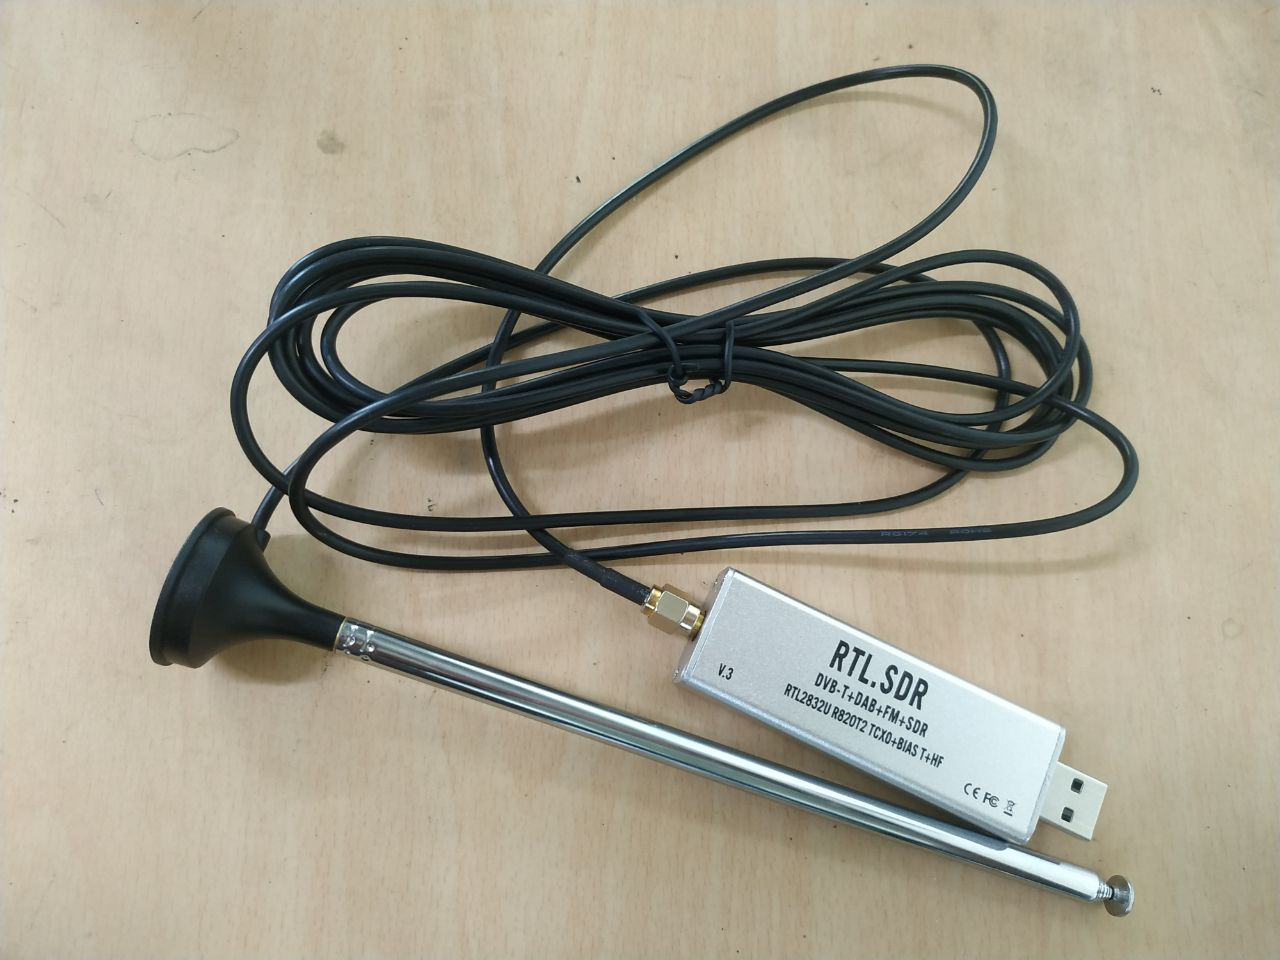
\includegraphics[width=0.5\columnwidth]{fm/rx/figs/rtl-sdr.png}
\caption{RTL-SDR}
\label{fig:rtl-sdr}
\end{figure}
\item Install and open GNU Radio using the following commands
\\
\begin{lstlisting}
sudo apt update
sudo apt install gnuradio
gnuradio-companion
\end{lstlisting}
\item How to construct the block diagram in GNU radio? \\
	\solution  \\
\textbf{Step-1}:\\
Search for Low pass filter block and add drag it to the work space.
\begin{figure}[H]
\centering
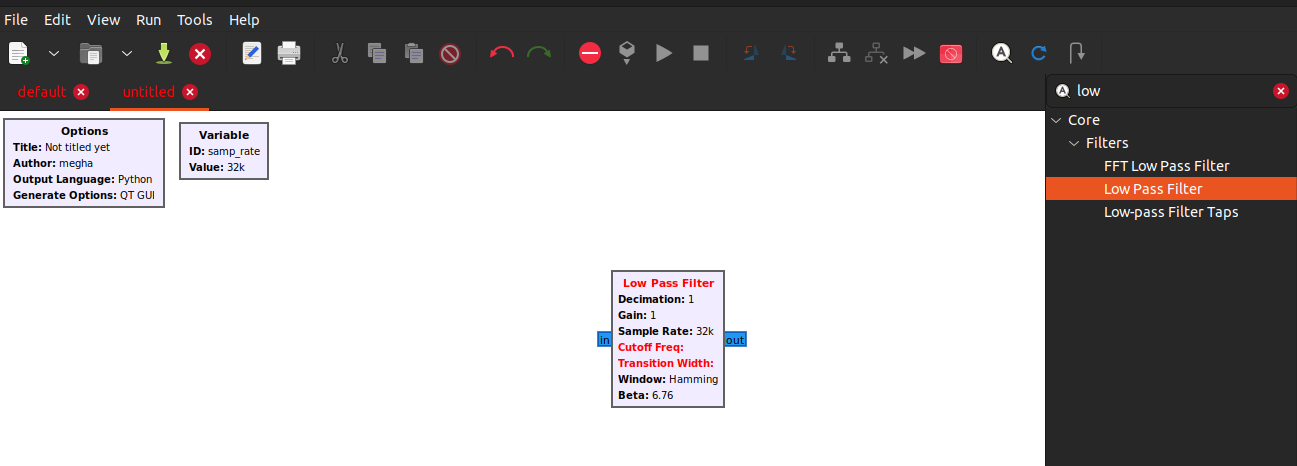
\includegraphics[width=\columnwidth]{fm/rx/figs/add.png}
\caption{Adding blocks}
\label{fig:add blocks}
\end{figure}
Similarly do for RTL-Source block,WBFM and Audio sink blocks.
\textbf{Step-2}:
Connect them according to the flowgraph shown in \figref{fig:Block_diagram}.
\begin{figure}[H]
\centering
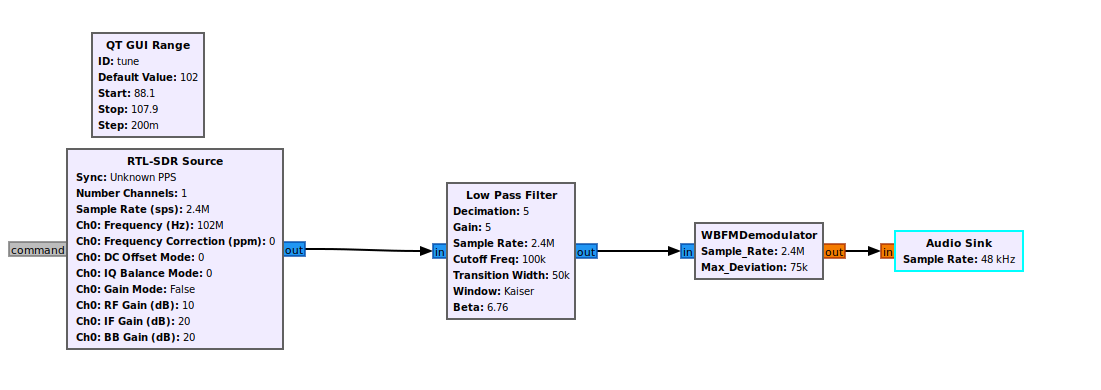
\includegraphics[width=\columnwidth]{fm/rx/figs/block_diagram.png}
\caption{Block diagram of GNU Radio}
\label{fig:Block_diagram}
\end{figure}
\textbf{Note}:
Refer the following website for any queries.
\begin{lstlisting}
https://wiki.gnuradio.org/index.php?title=Creating_Your_First_Block
\end{lstlisting}
\item Explain each block in block diagram \\
	\solution \\
\textbf{1. RTL-SDR Source}:\\
The RTL-SDR Source block is used to stream samples from RTL-SDR device.
\begin{figure}[H]
\centering
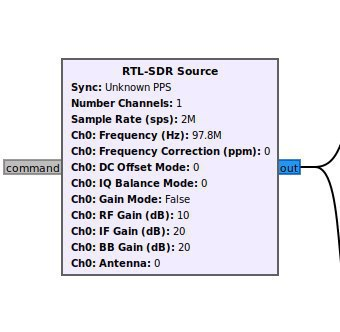
\includegraphics[width=0.4\columnwidth]{fm/rx/figs/source_block.png}
\caption{RTL-SDR Source Block}
\label{fig:source block}
\end{figure}
\textbf{2. Low Pass Filter}:\\
Low Pass Filter removes frequencies that are higher than the cutoff.
\begin{figure}[H]
\centering
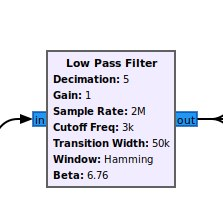
\includegraphics[width=0.3\columnwidth]{fm/rx/figs/lpf_block.png}
\caption{Low Pass Filter Block}
\label{fig:lpf}
\end{figure}
\textbf{3. WBFM}:\\
WBFM Receive is a block for demodulating a broadcast FM signal. The output is the demodulated audio.
\begin{figure}[H]
\centering
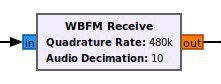
\includegraphics[width=0.3\columnwidth]{fm/rx/figs/wbfm_block.png}
\caption{WBFM Block}
\label{fig:wbfm block}
\end{figure}
\textbf{4. Audio sink}:\\
Audio Sink block provides audio output signal at the computer speakers.
\begin{figure}[H]
\centering
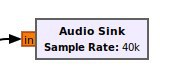
\includegraphics[width=0.3\columnwidth]{fm/rx/figs/audio_sink.png}
\caption{Audio Sink Block}
\label{fig:audio sink block}
\end{figure}
Connect the RTL-SDR to the system and execute the flowgraph in \figref{fig:Block_diagram}.\\
We can listen to the sound which we have transmitted.\\
A default python code is generated and stored as
\begin{lstlisting}
fm/rx/codes/fm_receiver.py
\end{lstlisting}
\item How to replace LPF default code with custom code?\\
\solution \\
\textbf{Step-1}:
Disable Low pass filter block and search for the python block and add it to the workspace.
\begin{figure}[H]
\centering
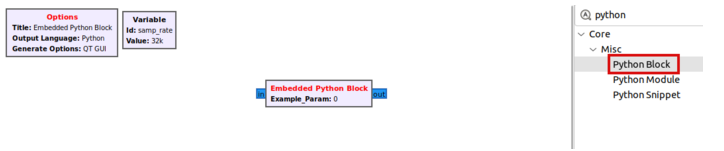
\includegraphics[width=\columnwidth]{fm/rx/figs/step_1.png}
\caption{search for blocks}
\label{fig:search for blocks}
\end{figure}
\textbf{Step-2}:
Double-click the block to edit the properties as in \figref{fig:Edit properties}
\begin{figure}[H]
\centering
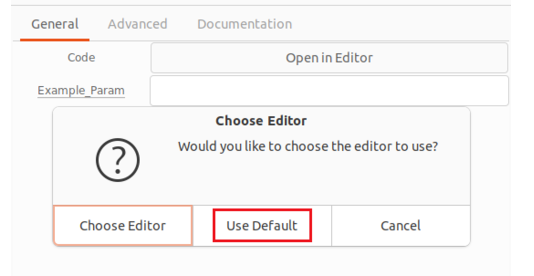
\includegraphics[width=0.7\columnwidth]{fm/rx/figs/step_2.png}
\caption{Edit properties}
\label{fig:Edit properties}
\end{figure}
\textbf{Step-3}:
Change the block name as required by editing in the code as shown in \figref{fig:changing block name}                                               
\begin{figure}[H]
\centering
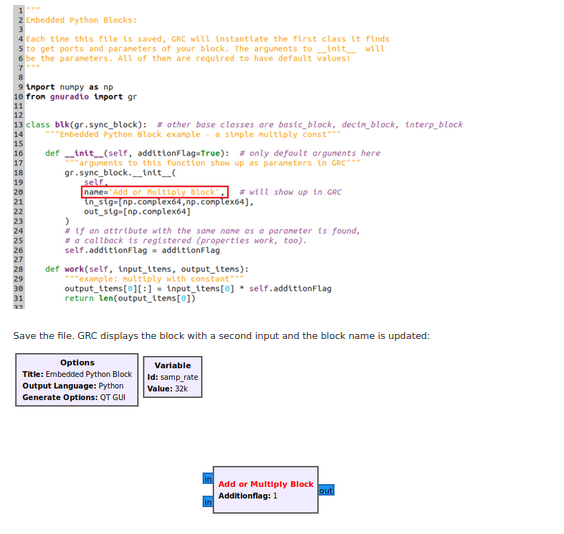
\includegraphics[width=\columnwidth]{fm/rx/figs/step_3.png}
\caption{Changing block name}
\label{fig:changing block name}
\end{figure}
\textbf{Step-4}:
Change the parameter name as required by editing in the code as shown in \figref{fig:changing parameter name}                                               
\begin{figure}[H]
\centering
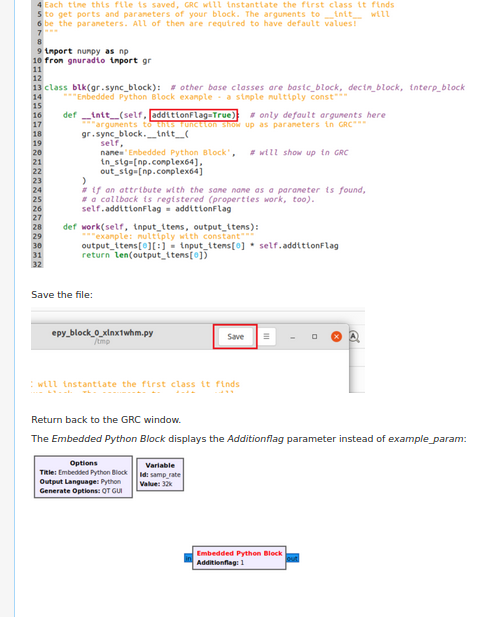
\includegraphics[width=0.7\columnwidth]{fm/rx/figs/step_4.png}
\caption{Changing parameter name}
\label{fig:changing parameter name}
\end{figure}
Replace the below code with default code
\begin{lstlisting}
fm/rx/codes/lpf_block.py
\end{lstlisting} 
\item Read the data from RTL SDR using python code and without using GNU radio.
\\
\solution \\
The following code reads the data from RTL-SDR without GNU radio.
\begin{lstlisting}
fm/rx/codes/source_own.py
\end{lstlisting}
\item Design Low pass filter block without using GNU Radio
\\
\solution \\
The following code works as low pass filter.
\begin{lstlisting}
fm/rx/codes/lpf_own.py
\end{lstlisting}
\end{enumerate}